\documentclass[usenatbib]{mnras}
\usepackage{siunitx}
\usepackage{graphicx}	% Including figure files
\usepackage[utf8]{inputenc}
\usepackage[english]{babel}
\usepackage{float}
\usepackage{amssymb, amsmath, yhmath}
\usepackage{verbatim}

\newcommand{\expect}[2]{\left< #1 \right| #2 \left| #1 \right>}
\renewcommand{\d}[1]{\! \mathrm{d}#1 \:}
\newcommand{\deriv}[2]{\frac{\d{#1}}{\d{#2}}}
\newcommand{\pderiv}[2]{\frac{\partial{#1}}{\partial{#2}}}
\newcommand{\parsq}[2]{\frac{\partial^2{#1}}{\partial{#2}^2}}

\bibliographystyle{apa}
\setlength{\bibhang}{1in}
\setcitestyle{authoryear, open={(},close={)}}
\renewcommand{\bibsection}{\section*{References}}

\usepackage{graphicx}

\newcommand{\squote}[1]{\lq #1\rq}

\renewcommand{\d}[1]{\ensuremath{\operatorname{d}\!{#1}}}
\newcommand{\poweV}[1]{\SI{e#1}{\electronvolt}}
\newcommand{\ineV}[2]{\SI{#1 e #2}{\electronvolt}}
\newcommand{\lcdm}{$\Lambda$CDM}
\DeclareSIUnit\parsec{pc}
\DeclareSIUnit\lightyear{ly}
\DeclareSIUnit\year{yr}
\begin{document}

\title[Dark Matter Heating]{Heating of Milky Way Disk Stars by Dark Matter Fluctuations in Cold Dark Matter and Fuzzy Dark Matter Paradigms}
\author[B. V. Church and J. P. Ostriker]{
Benjamin V. Church, \thanks{Contact e-mail: bvc2105@columbia.edu}
Jeremiah P. Ostriker,$^{1}$ \thanks{Contact e-mail: jpo@astro.columbia.edu}
\\
$^{1}$Columbia University, Department of Astronomy, New York, NY 10025, USA.}
\maketitle
\begin{abstract}
Although highly successful on cosmological scales, Cold Dark Matter (CDM) models predict unobserved over-dense \squote{cusps} in dwarf galaxies and overestimate their formation. We consider a popular modification to CDM particle physics involving an ultra-light axion-like scalar boson which promises to reduce these observational discrepancies at galactic scales. The model, known as Fuzzy Dark Matter (FDM), avoids cusps, suppresses small-scale power, and delays galaxy formation via macroscopic quantum pressure. We compare the substructure of galactic dark matter halos comprised of ultra-light axions with masses $\poweV{-24} \leq m_p \leq \poweV{-18}$ to conventional CDM results. Besides self-gravitating subhalos, FDM includes additional substructure in the form of non-virialized over-dense wavelets formed by quantum interference patterns. Wavelets provide a more efficient source of heating to the galactic disk than subhalos. We provide analytical measures of substructure-induced perturbations and heating to interior test particles responsible for the thickening of galactic disks and tidal streams. FDM models with moderate particle masses produce a cumulative heating of $30\, \si{\kilo\meter\per\second}$ over an approximate galaxy lifetime of $10\, \si{\giga\year}$ corresponds to the velocity dispersion of the Milky Way population II stars. Comparing the best theoretical estimates for heating along with best fit parameters from FDM simulations to observations of the velocity dispersion of population II stars provides a lower bound on the FDM particle mass $m_p > 1.30 \times \SI{e-22}{\electronvolt}$.
\end{abstract}

\begin{keywords}
cosmology: theory -- dark matter -- galaxies: structure
\end{keywords}

\section{Introduction}
	Over-dense regions of dark matter collapse to roughly localized concentrations of matter called ‘halos’ which are well-described by spherically symmetric density profiles. However, compositionally identical halos may vary significantly from these profiles in small-scale power i.e. substructure. Simulations suggest that substructure forms clumps which are qualitatively similar to free dark matter halos. We adopt a substructure formalism which tracks subhalos as an estimate of total substructure. The secondary gravitational effects of these subhalos is dependent on the subhalo mass function and the shape of small halo profiles, which is directly dependent on properties of the dark matter physics under consideration.                
        The standard cosmological model (\lcdm) contains a massive electromagnetically non-interacting component known as Cold Dark Matter (CDM) with density parameter $\Omega_c = 0.259 \pm 0.006$. The properties of this substance are largely unknown and are assumed to be approximately that of a perfect fluid with negligible pressure compared to its energy density i.e. comprised of cold or non-relativistic matter. Constraints obtained from The Sloan Digital Sky Survey measurement of Ly-$\alpha$ forest power spectra and surveys of dwarf galaxies below the free-streaming scale rule out most models of relativistic (hot) matter as the primary component of dark matter \citep{can_neutrinos}. 
\par
        Although successful on cosmological scales, CDM models fail to make accurate predictions when compared with observations at distance scales less then \SI{10}{\kilo\parsec}. When compared with studies of dwarf galaxy rotation curves, CDM predicts unobserved density \squote{cusps} in the center of dark matter halos \citep{ultralight}. This failure is known as the \squote{cusp-core problem}. Another serious concern is the \squote{missing satellite problem}  \citep{missing_satellites}. The number of satellite galaxies predicted for a milky-way-like galaxy is greater than what we observe by an order of magnitude. This issue is sharpened by the \squote{too big to fail} problem of galaxy formation that claims some of the predicted satellites are so massive that it is impossible for them to not have any stars \citep{too_big_to_fail}. Various complex phenomena have been suggested as solutions to these problems such as baryonic feedback mechanisms which redistribute matter or  hypothetical dark matter self-interactions.

\par
	An alternative model gaining popularity known as Fuzzy Dark Matter (FDM) describes dark matter as comprised of ultra-light($m \approx \poweV{-22}$) bosons whose characteristic wavelength is on the order of $\SI{1}{\kilo\parsec}$. Such ultralight particles are possible in various theories beyond the standard model \citep{axion_cosmology}. In particular, the class of axion-like particles is a perfect candidate for FDM and therefore, we refer to the mass of the constituent particles of FDM as the axion mass $m_p$. Macroscopic quantum mechanical wave effects “smear” the density profile on scales less than $\sim \SI{1}{\kilo\parsec}$ which removes problematic cusps from the center of large halos. These cusps are replaced by dense self-gravitating quantum states known as soliton cores which may facilitate indirect observation evidence for FDM. Furthermore, the quantum mechanical pressure caused by the large wavelength of FDM suppresses the formation of low-mass halos and entirely eliminates the formation of any halo or subhalo smaller than this wavelength, reducing or eliminating the missing satellites problem. Significant further effort remains in determining further discrepancies between FDM and CDM and whether these can, in conjunction with observational constraints, rule out one or both of the models.
 
\par
        The dynamical effects of CDM have been studied in some detail, especially regarding the accretion and tidal stripping of CDM subhalos by large galaxies and their associated dark matter halos. On the other hand, research on the dynamics of FDM distributions is in its infancy. However, dynamical studies have focused on simulations which inherently have a fixed resolution and thus artificially suppress small-scale power. In this paper, we present analytic estimates for substructure dynamical fluctuations which do not suffer from limited resolution. The resolution limit of simulations causes underestimates to subhalo populations and therefore to their dynamical effects. 
\par 
	CDM and FDM models predict significant differences in the distribution of halo substructure. The FDM subhalo mass function is zero below a cutoff scale determined by the axion mass expressed by the Jean’s scale at which quantum pressure and gravitational attraction balance:
\setlength{\belowdisplayskip}{4pt} \setlength{\belowdisplayshortskip}{4pt}
\setlength{\abovedisplayskip}{4pt} \setlength{\abovedisplayshortskip}{4pt}

\begin{equation}
k_J = 66.5 \cdot (1+z)^{1/4} \left( \frac{\Omega_a h^2}{0.12} \right) \left(\frac{m_p}{\poweV{-22}} \right)^{1/2} \si{\per\mega\parsec}
\end{equation}

as given by \citet{axion_cosmology}. \\ For light axions, the subhalo mass function is significantly suppressed though the entire range of substructure for a halo comparable to the Milky Way’s. However, FDM subhalos will exhibit solitons which, for moderately-sized subhalos and large axion masses, are very dense and largely unaffected by tidal disruption. In addition, a surprising standing wave phenomenon has been observed in the density profiles produced by small-scale FDM computer simulations \citep{cold_and_fuzzy}. These standing waves, named wavelets, radically alter the dark matter profile and may through gravitational interactions disturb the baryonic components in directly measurable ways. The primary effect of these wavelets is to introduce time-varying perturbations to the gravitational potential on a much shorter time-scale than the evolution of primary structure after the system has come into virial equilibrium. 
\par
	The velocity dispersion of stars in a galactic disk provide a proxy of the gravitational perturbations produced by the dark matter halo substructure. We expect that dispersion increases with age via an approximate power law $\sigma \propto t^\beta$. Therefore, the best observational bounds will come from old population II stars.  

\section{Heating via Substructure Dynamics}

\subsection{Estimating The Heating Due to Transits}

We provide a rough analysis of the heating due to transiting over-dense regions of dark matter. Each transit causes a change in velocity of approximately,
\begin{equation}
v^2 = \frac{M_l G}{b v_l}
\end{equation}
where $M_l$ is the mass of the region, $v_l$ is its velocity, and $b$ is the distance at closest approach. However, the heating is only effective if these perturbations are adiabatic which approximately corresponds to the constraint,
\begin{equation} \label{adiabatic}
\frac{b}{v_l} < \frac{P}{2}
\end{equation}
where $P$ is the characteristic period of the objects subjected to perturbation, in this case the period for lateral oscillations through the galactic disk. The total heating is therefore given by the accumulation of all such encounters,
\begin{align}
\deriv{\sigma^2}{t} &= \int (2 \pi b) \: \d{b} \: n v_p \: \left( \frac{M_l G}{b v_p} \right)^2 
\\
& = \frac{M_l^2 G^2}{v_l} \: 2 \pi n \ln{\frac{b_{\mathrm{max}}}{b_{\mathrm{min}}}}
\end{align}
The maximum distance across which the heating is efficient is fixed by \ref{adiabatic} and the minimum distance is given by $r_l$,  the characteristic size for the perturbing objects. Furthermore, the period of oscillation out of a thin disk is given by the velocity dispersion and surface density of the disk via,
\begin{equation}
P = \frac{\sigma}{4 \pi G \Sigma}
\end{equation} 
Therefore, in terms of the overall one-dimensional velocity dispersion, we derive the time-dependent heating as,
\begin{align}
\deriv{\sigma^2}{t}  = \frac{M_l^2 G^2}{\sigma} \: 2 \pi n \ln{\frac{\sigma^2}{8 \pi G \Sigma r_l}}
\end{align}
A more detailed calculation detailed in \cite{milkywayblackholes} gives somewhat alterned numerical factors,
\begin{align} \label{heating}
\deriv{\sigma^2}{t} =\frac{8 \pi M_l^2 G^2}{V} \: n \: \ln{\frac{\sigma^2}{8 \pi G \Sigma r_l}}
\end{align}
where $V$ is the relative velocity between the disk stars and the transiting objects. An alternative approach is given by \cite{ultralight} which only considers the tidal effects on disk heating. This model assumes that only local dispersion can lead to overall heating. However if processes such as outgoing density waves are an inefficient means for disapating differential motions of the disk then dynamical friction between oscillating disk components will tend to dissipate oscillation energy into disk heating and therefore contribute to the thickening. In this analysis, we will assume that such processes are inefficient and therefore equation \ref{heating} gives a more reasonable estimate of the total rate of heating.  


\begin{comment}

\section{Monte Carlo Results}

\section{calculating the dynamical influence of substructure}

\subsection{RMS Fluctuations}
Given a halo and a description of its substructure  we wish to determine its effects on the evolution of the system especially the baryonic components. The dynamics of the substructure introduce time-varying potentials which cause test particles to disperse in energy. This effect may contribute to the thickening of galactic disks and tidal streams. To assess magnitude of these effects we examine the time dependence of the potential. The root-mean-square (RMS) fluctuation at a given point in the halo is calculated as:
\begin{equation}
F_{RMS} = \sqrt{\left< \left( \frac{\d{\phi}}{\d{t}} \right)^2 \right>} = \sqrt{\left< \left(\sum_{i = 1}^N{\frac{M_i(r)G}{r_i^2} \hat{r} \cdot \vec{v}_i} \right)^2 \right>}
\end{equation}

	We assume that the velocities of distinct halos and their directional unit vectors are uncorrelated. Under these assumptions, the expected value is the sum of the expected value of each term:
\begin{align} \label{fluc}
F_{RMS} &= \sqrt{\sum_{i = 1}^N{\left< \left(\frac{M_i(r)G}{r_i^2}\right)^2 \right> \left< \left(\hat{r} \cdot \vec{v}_i \right)^2\right>}} \\ &= \sqrt{\sum_{i = 1}^N{\sigma(R) \left< \left(\frac{M_i(r)G}{r_i^2}\right)^2 \right>}} 
\end{align}  where $\sigma(R_i)$ is the linear velocity dispersion at the halo's position. This sum is estimated via numerical integration in python 2.7 with scipy v. 0.17.0 using the distribution of subhalo masses and positions given by equations (\ref{dist}, \ref{trunc}). 
 

\begin{figure}
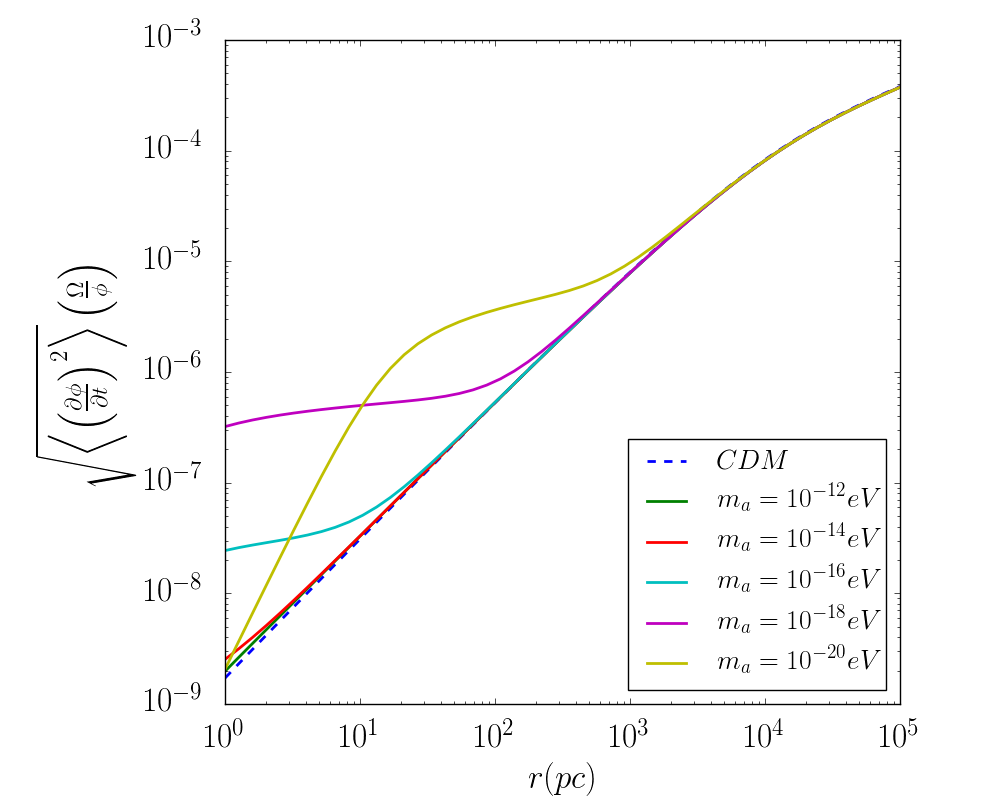
\includegraphics[width=\columnwidth]{High_Mass_Fluctuatations.png}
\vspace*{-5mm}
\caption{RMS fluctuations normalized to local host gravitational potential and orbital period as a function of radius for various dark matter models with $m_p$ in the range \SIrange{e-12}{e-20}{\electronvolt}.}
\label{fig:highfluc}
\end{figure}

\begin{figure}
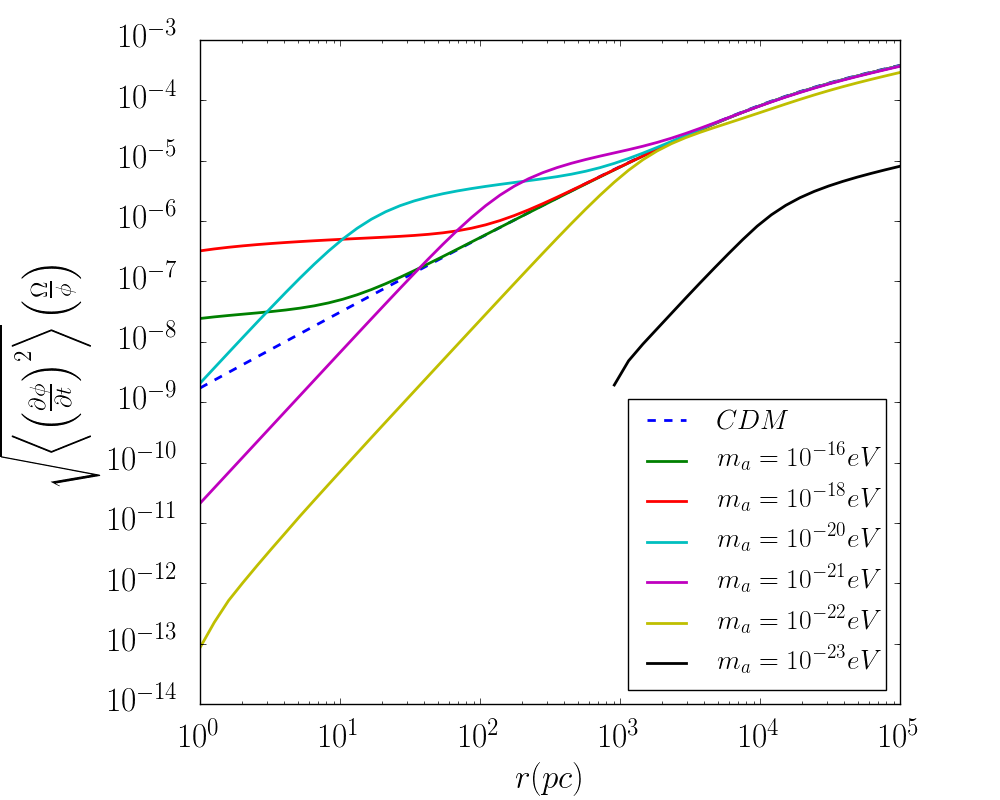
\includegraphics[width=\columnwidth]{Normed_Fluctuations.png}
\vspace*{-5mm}
\caption{RMS fluctuations normalized to local host gravitational potential and orbital period as a function of radius for various dark matter models with $m_a$ in the range \SIrange{e-16}{e-23}{\electronvolt}.}
\label{fig:normfluc}
\end{figure}

\begin{figure}
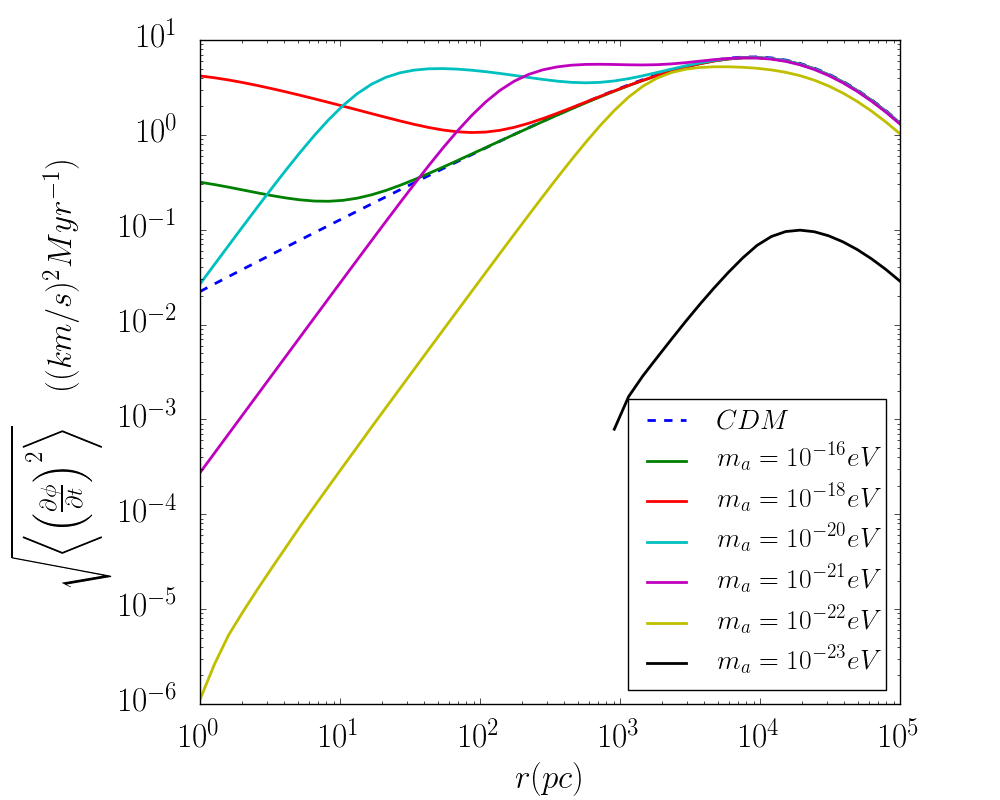
\includegraphics[width=\columnwidth]{Fluctuations.png}
\vspace*{-5mm}
\caption{Raw RMS fluctuations in \si{\kilo\metre\squared\per\second\squared\per\mega\year} as a function of radius for various dark matter models with $m_a$ in the range \SIrange{e-16}{e-23}{\electronvolt}.}
\label{fig:normfluc}
\end{figure}


\par
	In this paper, we present results for a halo with $M_p = 10^{12} M_{\odot}$ similar to the halo surrounding the Milky Way. Figure \ref{fig:highfluc} illustrates that for large axion masses, the FDM and CDM results are indistinguishable. This is an important consistency check of our calculations considering that CDM is the classical high-mass limit of FDM. However, as the mass of the axion increases, the fluctuations at small radii increase above their CDM counterpart. For a relatively heavy axion ($m_p > \poweV{-20}$), the suppression of small halos is insignificant and the solitons of subhalos are very dense, therefore the subhalos are less prone to tidal disruption. As the axion mass is further decreased, the number of small subhalos is significantly suppressed and the radius at which tidal effects completely disrupt solitons increases. For $m_p = \poweV{-23}$ all subhalos are completely tidally destroyed if $r < \SI{1}{\kilo\parsec}$ (see Figure \ref{fig:normfluc}). In the range \SIrange{e-16}{e-20}{\electronvolt}, FDM fluctuations exceed those of CDM for a $10^{12} M_{\odot}$ primary halo. Lighter axions drastically reduce all fluctuations due to the suppression of small scale structure.  

\subsection{Fourier Power Spectrum}
We study the power spectrum of
the fluctuations in the gravitational
potential by approximating the path of each subhalo as a straight line over the interaction window. This approximation is only valid for small fast-moving subhalos but the orbital radii are large compared with the subhalo radii. Further study will improve this result. Under this approximation:
\begin{equation}
\tilde{\phi}(\omega) = \frac{1}{\sqrt{2\pi}}\int_{-\infty}^{\infty} \! \frac{M\left(\sqrt{b^2 + (vt)^2}\right)G}{\sqrt{b^2+(vt)^2}} e^{-i \omega t}\d{t}
\end{equation}
\\ \\

\begin{figure}
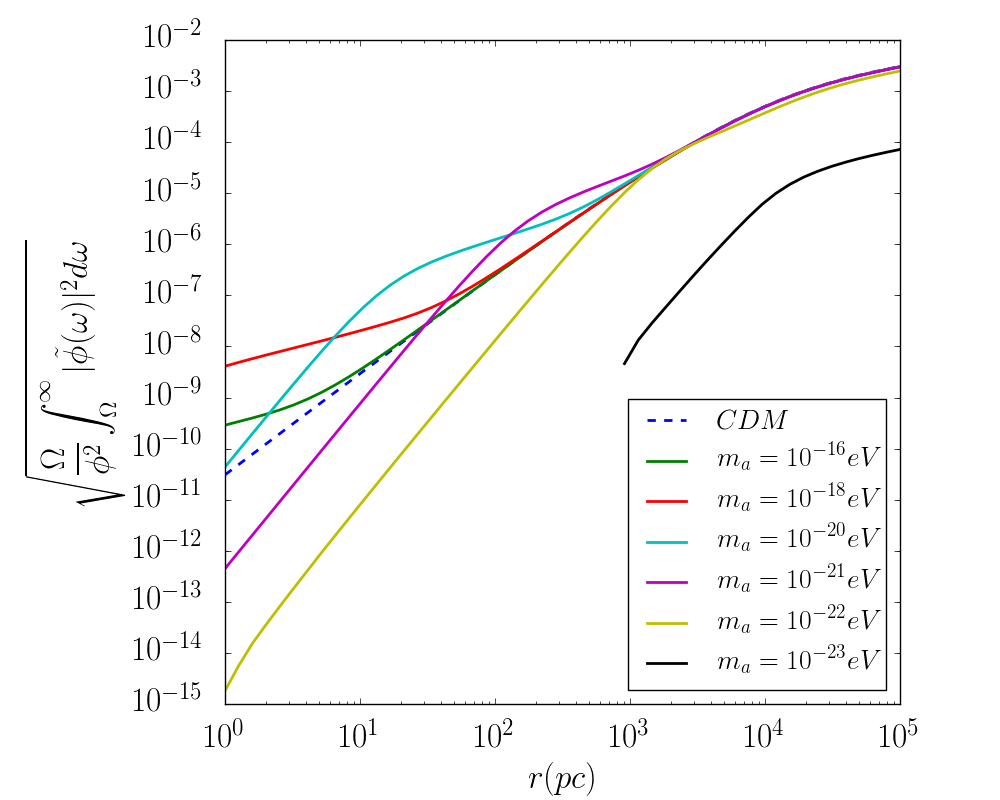
\includegraphics[width=\columnwidth]{Non-Adiabatic_Amplitude.png}
\vspace*{-5mm}
\caption{Non-adiabatic amplitude as a function of radius for various dark matter models with $m_a$ in the range \SIrange{e-16}{e-23}{\electronvolt}.}
\label{fig:fourierfluc}
\end{figure}

This integral is intractable when $b < r_{max}$ and must be computed numerically. However, when $b \geq r_{max}$,
\begin{equation}
\tilde{\phi}(\omega) = \frac{MG}{v} f_F\left(\frac{\omega b}{v} \right)
\end{equation} where
\begin{equation}
f_F(u) = \frac{1}{\sqrt{2\pi}} \int_{-\infty}^{\infty} \! \frac{e^{-iut'}}{\sqrt{1 + t'^2}} \d{t'} = \sqrt{\frac{2}{\pi}} K_0(u)
\end{equation}
Summing the power spectra of each halo,
we arrive at an approximate power
spectrum for the total fluctuations in
gravitational potential at a given point:
\begin{equation}
\left<\left| \tilde{\phi}(\omega) \right|^2 \right> = \left< \sum_{i = 1}^N \left(\frac{M_iG}{v_i} f_F\left(\frac{\omega b_i}{v_i} \right)\right)^2 \right>
\end{equation} 


The magnitude is normalized to the local
gravitational potential of the primary halo
and the frequency variable is normalized to
the local orbital period. This spectra is
summarized by integrating
over the power in high-frequency
(greater than orbital period) perturbations:
\begin{align}
P_{\Omega} &= \int_{\Omega}^{\infty} \! \left<\left| \tilde{\phi}(\omega) \right|^2 \right> \d{t} \\ &= \left< \sum_{i = 1}^N \left(\frac{M_iG}{v_i}\right)^2 \int_{\Omega_i}^{\infty} \! f_F\left(\frac{\omega b_i}{v_i} \right)^2 \d{\omega} \right> \\
&= \left< \sum_{i = 1}^N \left(\frac{M_iG}{v_i}\right)^2 \Omega_i \: F\! \left(\frac{\Omega b_i}{v_i} \right) \right>
\end{align} where 
\begin{equation}
F(u) = \frac{1}{u} \int_{u}^{\infty}\!\!\!\!\! f_F(x)^2 \d{x} = \frac{1}{u} \left[ G_{2, 4}^{3, 1} \left( \begin{smallmatrix} 1, \: \: 1 \\ \small\frac{1}{2}, \: \small\frac{1}{2}, \: \small\frac{1}{2}, \: 0 \end{smallmatrix} \Big| x, \: \frac{1}{2} \right) \right]^{\infty}_{u}
\end{equation}
$P_{\Omega}$ provides a measure of the total power in non-adiabatic perturbations which would
disperse orbiting test particles.

\end{comment}

\subsection{Heating in CDM}

\subsubsection{Spatial Profile}

	We model substructure as comprised entirely of subhalos which act as distinct massive particles subject only to gravitational attraction and tidal disruption. Following \citet{tidal_limit, unified_model} we adopt a
simplified model of CDM subhalo
formation and dynamics. The shape of
the subhalo mass function is assumed to
be spatially invariant, i.e. the position
and mass variables are decoupled. The
total density of subhalos is assumed to
follow the Navarro--Frenk--White (NFW) profile:
\begin{equation}
\rho(r) = \frac{\rho_0}{r/r_c (1+r/r_c)^2}
\end{equation} which also
describes the density profile of the
primary dark matter halo given by \citet{structure} from CDM simulations. This profile is fairly universal for the halos of massive cold particles which we assume accurately describe subhalos.

\subsubsection{Unresolved Mass Function}

	As the primary halo forms, it captures subhalos via accretion. The unresolved subhalo mass function refers to the distribution of subhalo masses at the time of accretion before dynamical effects such as tidal stripping have biased the distribution. We assume the unresolved subhalo mass function is very close in shape to the free halo mass function truncated above the primary halo mass. Based on simulations given by \citet{dark_wave} we take this fraction to be $\sim 10\%$. The CDM halo mass function and corresponding subhalo mass function calculated from simulations \citep{pop_of_subhalos, unified_model} are well fit by a power law: 
\begin{equation}
\frac{\d{n}}{\d{\: \ln{m_{acc}}}} = C \left(\frac{\rho(r)}{M_p}\right) \left(\frac{m_{acc}}{M_p} \right)^{-p} 
\end{equation}
with $p = 0.9$ and where $M_p$ is the mass of the primary or host halo. The equivalent for FDM is calculated numerically via an equivalent process. The halo mass function is calculated numerically from the Press--Schechter formalism \citep{substructure_FDM, marsh} and the soliton profile is fitted from simulations by \cite{schive_solitons}. 
\par

	Furthermore, we fix the total mass in (accreted) halos as a fraction of the total mass of the primary halo. Therefore,
\begin{align}
M_{\mathrm{halos}} & = \int m \deriv{n}{(\ln{m})} \d{(\ln{m})} \d{V}
\\
& = C \int \left(\frac{\rho(r)}{M_p}\right) \left(\frac{m}{M_p} \right)^{-p} \d{m} \d{V} 
\\
& = \frac{C}{1-p} \left[ \frac{(f_2 M_p)^{1-p}}{M_p^{-p}} \right] = f_1 M_p 
\end{align} 
so we fix the constant,
\begin{equation}
C = (1 - p)\frac{f_1}{f_2^{1-p}} 
\end{equation}

\subsubsection{Tidal Disruption} 

	We adopt a simplistic model of tidal stripping which underestimates the total effect. A tidal radius is calculated by setting the tidal force on a test mass equal to the gravitational attraction of the subhalo. The resulting radius is:
\begin{equation}
R_t = R \left(\frac{m_{acc}}{2M_p(R)}\right)^{1/3} =  R_{max} \left(\frac{m_{acc}}{M_p}\right)^{1/3} f_T(R)
\end{equation} 
with $f_T(R) \propto R/R_c(\ln(1+R/R_c) - R/(R+R_c))^{-1/3}$ where $R_c$ is the core radius of the primary halo. We then suppose that total truncation occurs outside this radius and no disruption occurs within it. Thus,
\begin{equation}
\frac{m}{m_{acc}} = 
\begin{cases}
    \frac{\ln{(1+R_t/r_c)} - R_t/(r_c+R_t)}{\ln{(1+c)} - c/(1+c)},& \text{if } R_t < r_{max}\\
    1,              & \text{otherwise}
\end{cases}
\end{equation} 
However, $m_{acc} = 200 \rho_0 \frac{4}{3} \pi c(m)^3 r_c^3$ and $r_{max} = c(m) \: r_{c}$ so 
\begin{equation}
R_t = r_{max} f_T(R)
\end{equation}
\begin{equation} \label{trunc}
T_R(m_{acc}) =  \frac{m}{m_{acc}} = 
\begin{cases}
    \frac{\ln{(1 + x)} - x/(1 + x)}{\ln{(1+c)} - c/(1+c)},& \text{if } f_T(R) < 1\\
    1,              & \text{otherwise}
\end{cases}
\end{equation} where $x = c(m) \cdot f_T(R)$. Since $c$ is a weak function of $m$, the remaining mass fraction is also a weak function of $m$. Therefore, even the final resolved subhalo mass function is approximately decoupled in mass and radius, in agreement with the results of \citet{unified_model}. Tidal disruption in the FDM case is similar, the density profile is truncated at the tidal radius. However, since the mass and radius of a soliton are inversely related \citep{solitons}, if the tidal radius is less than the soliton radius a runaway process will completely disrupt the halo. This is because as mass is stripped from the soliton, the soliton grows due to quantum pressure (previously halted by gravitational attraction) which pushes more mass outside the tidal radius. Due to the solitonic cores in FDM, the remaining mass fraction after tidal disruption is strongly dependent on the subhalo mass because the shape of the soliton profile and behavior are strongly mass-dependent. 


\subsubsection{Calculating the Heating}
Using the quantities we derived earlier and using the approximation $V \approx \sqrt{3} \sigma_H$,
\begin{equation}
\deriv{\sigma^2}{t} = \frac{8 \pi}{\sqrt{3} \sigma_H} \int T_R(m)^2 (m G)^2 \deriv{n}{m}  \ln{\frac{\sigma_H^2}{8 \pi G \Sigma r(m)}} \d{m}
\end{equation}
For a Milky Way-like halo with $M_p = 10^{12} \, M_\odot$, we can calculate the level of heating as a function of radius where we assume that $\Sigma = \Sigma_0 e^{-r/r_0}$. (CITATION NEEDED?) For the Milky Way, we take $r_0 = 5 \si{\kilo\parsec}$. If we assume that the primary halo and substructure formed quickly on the scale the lifetime of the disk, then the time dependence of the heating rate is given by,
\begin{equation}
\deriv{\sigma^2}{t} \propto \sigma^{-1} \ln{\sigma^2} 
\end{equation} 
which implies that $\beta \approx \frac{1}{3}$ for the time dependence $\sigma \propto t^\beta$. 

\subsection{Heating in FDM}

The fluctuations due to subhalos dynamics are reduced in FDM compared to CDM because the halo mass function is suppressed at low mass and light subhalos are more easily tidally disrupted via a runaway soliton reformation effect. However, there is an added contribution due to interference of excited modes which produce time dependence over-density known as wavelets. We assume that the density of the wavelets is a fixed multiple of the local mean density. Using results from Philip Mocz (CITATION NEEDED),
\begin{equation}
M_w = A \left(\frac{\lambda}{2} \right)^3 \rho(r) 
\end{equation}  
where $\lambda$ is the local characteristic scale. We also assume that entire mass of the primary FDM halo forms the wavelets which gives, $M_w n = \rho(r)$. However, because these wavelets are inherently produced by quantum mechanical interference, they will approximately saturate the uncertainty relations such that,
\begin{equation}
\lambda m_p \sigma_H \approx \hbar
\end{equation}
where $m_p$ is the particle mass. 
A more careful calculation given by Philip Mocz (CITATION NEEDED) shows that,
\[ \lambda = \frac{ 2 \pi \hbar}{m_p \sigma_H \sqrt{\frac{3}{2}}} \]
Therefore, the heating due to wavelets is approximately given by,
\begin{equation}
\deriv{\sigma^2}{t} = \frac{A \pi}{2^{3/2}} \left( \frac{h}{m_p} \right)^3 \frac{(\rho(r) G)^2}{\sigma_H^4} \ln{\frac{m_p\sigma_H^3}{8 \pi \hbar G \Sigma}}
\end{equation}
Therefore, using $\Sigma = \Sigma_0 e^{-r/r_0}$ we can express the rate of heating as a function of radius. Furthermore, if we assume that the primary halo and substructure formed quickly on the scale the lifetime of the disk, then the time dependence of the heating rate is given by,
\begin{equation}
\deriv{\sigma^2}{t} \propto \sigma^{-4} \ln{\sigma^2} 
\end{equation} 
which implies that $\beta \approx \frac{1}{6}$ for the time dependence $\sigma \propto t^\beta$. 

\begin{figure}
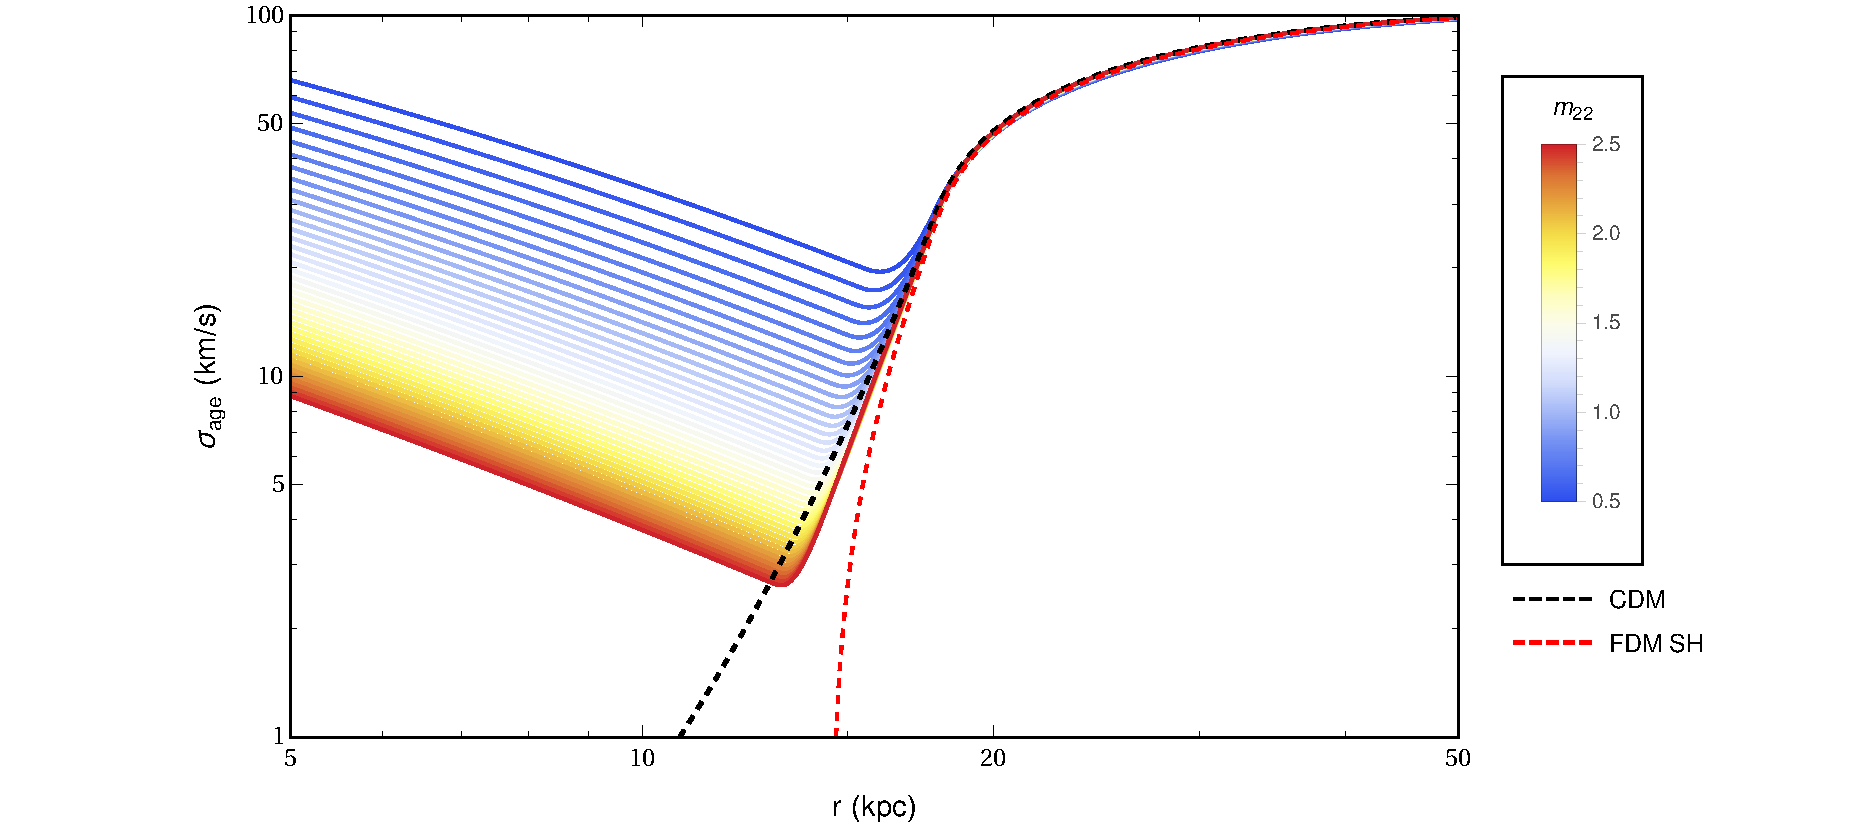
\includegraphics[width=\columnwidth]{FDM_velocity}
\vspace*{-5mm}
\caption{Rate of heating due to wavelets as a function of radius for axion masses $m_{a}$ in the range \SIrange{0.25 e-22}{ 1.75 e-22}{\electronvolt}. for a Milky Way-like halo with $M_p = 10^{12} \, M_\odot$ and $\Sigma_0 = 64 \, M_\odot \, \si{\per\parsec^2}$.}
\label{fig:radiusheating}
\end{figure}

\subsection{Scaling with Circular Orbit Velocity}


\begin{figure}
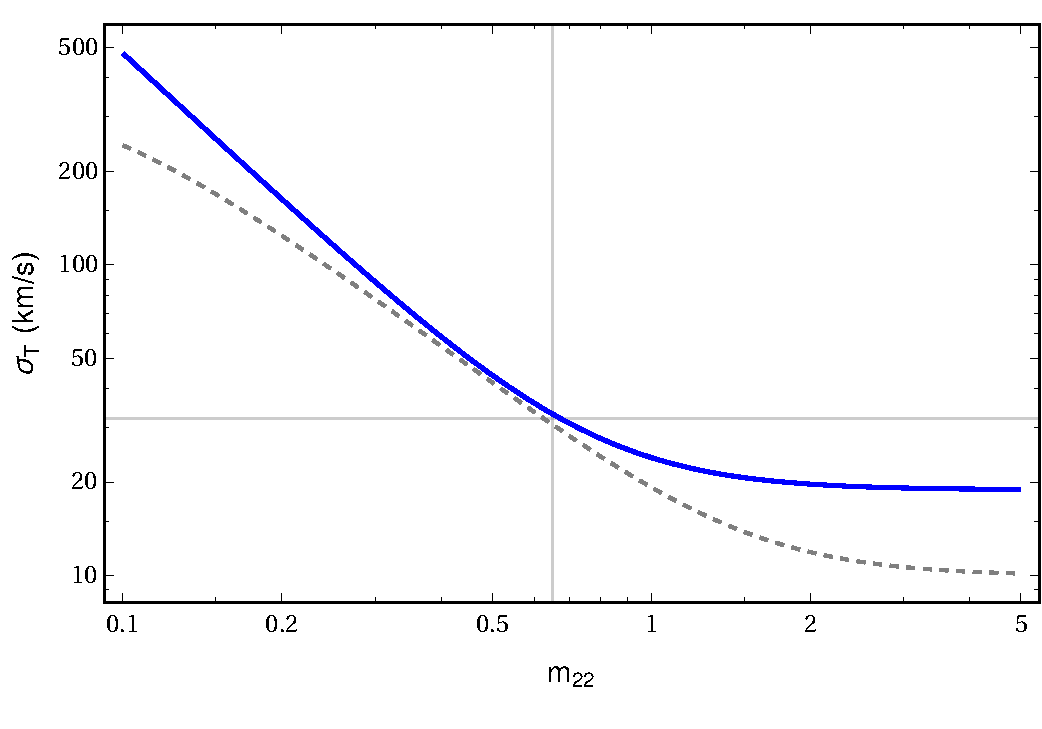
\includegraphics[width=\columnwidth]{FDM_mass_dep}
\vspace*{-5mm}
\caption{Rate of heating due to wavelets at $r = 8\, \si{\kilo \parsec}$ as a function of axion masses $m_{a}$ in the range \SIrange{0.1 e-22}{ 10 e-22}{\electronvolt}. for a Milky Way-like halo with $M_p = 10^{12} \, M_\odot$ and $\Sigma_0 = 64 \, M_\odot \, \si{\per\parsec^2}$. The horizontal line is fixed at $34\, \si{\kilo\meter\per\second}$, the observational maximum on velocity dispersion of the Milky Way population II stars. }
\label{fig:radiusheating}
\end{figure}


\section{Conclusion}


\subsection{Constraints on Particle Mass}

	The Milky Way has a thin disk of newer population I stars and a thick disk of older population II stars. The thick disk has velocity dispersion of approximately \SI{34}{\kilo\meter\per\second} in its thickest parts \citep{milky_way}. Therefore, the velocity dispersion caused by substructure heating cannot exceed this value. We find that CDM does not produce sufficient heating to be constrained by observational measurements of the Milky Way disk. However, the heating due to wavelets in FDM is strongly dependent on particle mass and far more efficient than other substructure. In the low-mass limit, the heating may vastly exceed observational bounds. Using the results quoted for population II stars as a strict cutoff, we derive a lower bound on the mass of the FDM particle,
\begin{equation}
m_p > 0.80 A^{1/3} \times \SI{e-22}{\electronvolt}
\end{equation}
Numerical simulations give the best estimate $A \approx 3.6$ (CITE PHILIP). Using this value, we obtain the most probable bound,
\[ m_p > 1.30 \times \SI{e-22}{\electronvolt} \]

\subsection{Comparison with WDM}

\section*{Acknowledgments}
We thank Mihir Kulakarni for his code to calculate the FDM halo mass function and his invaluable guidance on this project and Philip Mocz and Hsi-Yu Schive for helpful discussions about solitons and wavelets. Many thanks to Philip Mocz for providing the numerical factors determining the mass of a wavelet. We also thank Hsi-Yu Schive for providing simulation data. 

\bibliography{mybib}


 
\end{document}
